\subsecao{Theoretical Foundation}

\subsubsecao{Unmanned Aerial Vehicles (UAVs)}

Multirotor Unmanned Aerial Vehicles (UAVs), such as quadcopters, are widely adopted in aerial manipulation missions due to their Vertical Take-Off and Landing (VTOL) capability and their ability to maintain hovering flight. In the context of non-cooperative target capture, maintaining stable hovering flight and performing low-speed translation are essential mechanical requirements to ensure robotic gripper alignment and successful target approach \cite{cocuzza2021, meng2020, bonyan2018}.

To describe the dynamic and kinematic behavior of these aircraft, the literature relies on the Newton--Euler formalism, modeling the UAV as a rigid body. The mathematical formulation, as schematically illustrated in Fig.~\ref{fig:quadrotor_schematic}, requires the definition of two main coordinate systems: an inertial reference frame fixed to the Earth ($F_0$) and a moving reference frame attached to the robot's center of mass ($F_b$). The state of the aircraft in three-dimensional space has six Degrees of Freedom (6 DoF), consisting of three translational motions along the Cartesian axes ($x$, $y$, $z$) and three rotational motions, commonly expressed by the Euler angles: roll ($\phi$), pitch ($\theta$), and yaw ($\psi$) \cite{sciortino2018}.

\begin{figure}[H]
    \centering  

    \caption{Schematic view of the quadrotor: coordinates and motion principle}
    \label{fig:quadrotor_schematic}

    \vspace{0.1cm}

    \includegraphics[width=0.4\linewidth]{figuras/uav_reference_frames.png}

    \vspace{0.1cm}

    \begin{flushleft}
        \footnotesize Source: Navajas and Prada (2014), cited in Adriansyah, Sulle, and Minarso (2017).
    \end{flushleft}

\end{figure}

The directional rotation matrix that converts coordinates from the body reference frame to the inertial reference frame is fundamental for projecting thrust and velocity vectors. In this model, the rotational dynamics of the system are governed by the inertia matrices and by the torques resulting from differences in propeller rotation, also encompassing gyroscopic effects \cite{sciortino2018, cocuzza2021}.

The main complexity in the modeling and control of multirotor systems lies in the fact that they are under-actuated systems. Although they possess six Degrees of Freedom (6 DoF) of motion in space, the system operates with a smaller number of independent control inputs (usually grouped into total vertical thrust and roll, pitch, and yaw torques). The thrust force vectors generated by the rotors are strictly parallel to the vertical axis ($z$) of the aircraft body reference frame \cite{sciortino2018}. As a direct consequence of this physical geometry, the UAV is incapable of generating independent translational forces along the global horizontal axes ($x$ and $y$). To perform lateral or forward translation during target pursuit, the robot must necessarily rotate in roll or pitch, tilting its main thrust vector relative to gravity in order to project a force component in the direction of the desired motion \cite{sciortino2018, cocuzza2021}.

This kinematic constraint imposes strong coupling among the state variables, making the system highly nonlinear \cite{zhang2021}. This scenario becomes critical during the final moments of the mission, specifically during docking (physical coupling). Physical contact between the landing gear and the cage, together with the mechanical action of the robotic gripper, introduces impulsive disturbances such as unmodeled forces and torques, which abruptly affect the aircraft attitude \cite{cocuzza2021, ladig2021}. Coupled dynamics studies demonstrate that when the UAV control loop reacts to reject these disturbance torques by tilting the aircraft, the under-actuated characteristic causes undesirable horizontal displacements of the robot body, which may compromise gripper locking and result in capture failure \cite{cocuzza2021}.

To overcome these nonlinearities and ensure precise locking onto the cage handle, the UAV architecture requires the implementation of stabilization controllers structured in cascade or robust control schemes \cite{zhang2021}. In a cascade control scheme, the inner control loop must operate at a substantially higher frequency than the navigation loop, ensuring that small wind disturbances or contact impacts are rejected almost instantaneously. Obtaining this inertially damped platform is the fundamental engineering prerequisite to prevent abrupt oscillations of the onboard camera, enabling the deep learning algorithm and the outer Visual Servoing loop to operate on clear images until the final instant of locking. To enable the execution of this cascade control loop and guarantee the physical stability of the robot, the UAV hardware and software architecture is commonly divided into two processing levels: low-level inertial control and high-level mission processing \cite{shang2016, sciortino2018}.

To guarantee this stabilization under physical contact, low-level processing is managed by an onboard Flight Control Unit (FCU), with the Pixhawk system being one of the most established hardware platforms in the literature for this purpose \cite{shang2016}. The controller acts as the aircraft's central processing unit, executing highly reliable open-source firmware, such as PX4 or ArduPilot \cite{sciortino2018}. The interconnection of this system, as illustrated in the block diagram in Fig.~\ref{fig:pixhawk_architecture}, begins with the reading of critical sensors by the Pixhawk, such as the Inertial Measurement Unit (IMU), which calculates the instantaneous attitude of the robot at high frequencies. Based on these data, the FCU computes the correction and sends PWM signals to the Electronic Speed Controllers (ESCs). In turn, the ESCs modulate the rotation of the brushless motors to correct the UAV attitude and reject disturbances almost instantaneously \cite{sciortino2018}. It is the robustness of this internal hardware loop that guarantees the robot's mechanical support, preparing it to receive high-level navigation commands.

\begin{figure}[H]
\centering

\captionsetup{justification=centering}

\caption{Block diagram of the UAV low-level hardware architecture, illustrating the signal flow from inertial sensing to the mechanical actuation of the motors}
\label{fig:pixhawk_architecture}

\vspace{0.3cm}

\begin{tikzpicture}[scale=0.9, transform shape]

\tikzset{
block/.style={
draw=violet,
fill=violet!8,
thick,
rounded corners,
minimum width=6cm,
minimum height=1.6cm,
align=center
},
labelbox/.style={
fill=gray!15,
inner sep=3pt
}
}

\node[block] (imu)
{
Sensors / IMU\\
(Acceleration + Angular Velocity)
};

\node[labelbox, below=0.6cm of imu]
(data)
{Inertial data};

\node[block, below=1cm of data]
(fcu)
{
FCU / Pixhawk\\
(ArduPilot or PX4)\\
State Estimation + Control
};

\node[labelbox, below=0.6cm of fcu]
(pwm)
{PWM signals};

\node[block, below=1cm of pwm]
(esc)
{
ESCs\\
(Electronic Speed Controllers)\\
PWM modulation
};

\node[labelbox, below=0.6cm of esc]
(power)
{Modulated electrical power};

\node[block, below=1cm of power]
(motor)
{
Brushless Motors\\
Thrust Generation\\
(Mechanical actuation)
};

\draw[->, thick] (imu) -- (data);
\draw[->, thick] (data) -- (fcu);

\draw[->, thick] (fcu) -- (pwm);
\draw[->, thick] (pwm) -- (esc);

\draw[->, thick] (esc) -- (power);
\draw[->, thick] (power) -- (motor);

\end{tikzpicture}

\vspace{0.2cm}

\begin{flushleft}
\footnotesize Source: Prepared by the author (2026).
\end{flushleft}

\end{figure}

\subsubsecao{Computer Vision Applied to UAVs}

To ensure the autonomous approach and capture of a non-cooperative target, the visual perception system of the UAV acts as the primary means of identification and state estimation within the environment. Historically, object detection relied on classical computer vision methods based on color segmentation or the search for predefined visual patterns \cite{zhao2019}. In the HSV color model, for example, the image is processed by separating hue, saturation, and value in an attempt to isolate the target through contrast. Another widely adopted strategy consisted of designing algorithms to map geometric patterns, such as edges, corners, and specific textures, using traditional mathematical descriptors such as SIFT, SURF, or HOG \cite{amjoud2023, zhao2019}.

Specifically regarding these geometric descriptors, object detection was performed through sequential image scanning, analyzing the image in blocks using the sliding window technique. Each block was then processed by classification models, such as Support Vector Machines (SVM), to mathematically determine the probability that the object was contained within that region \cite{amjoud2023, zhao2019}. The main challenge of this approach is that recognition rules needed to be rigidly modeled by the developers. Furthermore, the requirement to traverse thousands of candidate windows within the same image to locate the target generated a high computational cost, making the system inefficient and redundant for robotic applications \cite{zhao2019}.

However, when deployed onboard UAVs operating in real-world scenarios, exposed to variable sunlight conditions and complex background environments, these methods face the problem known as the semantic gap \cite{zhao2019}. This gap represents the inability of the algorithm to convert combinations of basic pixel and line patterns into a robust and abstract representation of the object. Consequently, the system tends to confuse the target with environmental noise, reflections, or shadows \cite{zhao2019}.

To overcome the limitations of classical perception, the literature adopted Deep Learning through Convolutional Neural Networks (CNNs). In the domain of object detection, these architectures are predominantly divided into two-stage detectors (region proposal-based methods, such as Faster R-CNN) and single-stage detectors \cite{zhao2019, amjoud2023, terven2023}. Although two-stage models provide high accuracy, their elevated computational cost and latency make real-time execution infeasible on the limited onboard computing platforms of UAVs \cite{amjoud2023}.

Seeking to balance speed and accuracy, single-stage alternatives such as SSD (Single Shot MultiBox Detector) and CenterNet became popular. However, SSD presents inherent difficulties in detecting small targets and under significant scale variations \cite{amjoud2023}, while CenterNet, despite its anchor-free architecture, lacks robustness in feature extraction under highly dynamic backgrounds \cite{xiuling2024}. In parallel, the rise of Vision Transformers (ViTs) and models such as DETR (Detection Transformer) introduced substantial advances in global context understanding, mitigating the semantic gap \cite{amjoud2023}. However, the high computational load of these attention-based architectures significantly reduces the frame rate (FPS) on embedded Low-SWaP hardware, making their use impractical in high-frequency Visual Servoing critical control loops \cite{rawat2026}.

Due to these hardware constraints and the requirement for uninterrupted tracking, the YOLO (You Only Look Once) family of algorithms has become established as the state of the art for aerial robotics. Unlike its predecessors, YOLO formulates detection as a unified spatial regression problem, extracting feature maps and predicting bounding box coordinates together with class probabilities in a single forward pass through the network \cite{amjoud2023, afifah2025}. Figure~\ref{fig:yolo_architecture} illustrates the conceptual principle of this architecture, demonstrating how the original image is divided into a spatial grid to perform direct bounding box regression and classification simultaneously \cite{redmon2016}.

\begin{figure}[H]
    \centering

    \captionsetup{justification=centering}

    \caption{Fundamental detection architecture of the YOLO family, illustrating the division of the image into spatial grids and the direct regression of bounding boxes}
    \label{fig:yolo_architecture}

    \vspace{0.2cm}

    \includegraphics[width=0.8\linewidth]{figuras/yolo_architecture.png}

    \vspace{0.2cm}

    \begin{flushleft}
        \footnotesize Source: Redmon et al. (2016).
    \end{flushleft}

\end{figure}

Within the YOLO family, the YOLOv8 architecture represents an evolution over previous versions in terms of efficiency by adopting an anchor-free detection mechanism. By eliminating the use of predefined anchor boxes, the network simplifies the training process and reduces dependence on parameters associated with anchor boxes, favoring adaptation to object scale variations, a recurring phenomenon during the rapid approach of the UAV toward the target \cite{afifah2025}. In its lighter and optimized variant, YOLOv8n (Nano), the architecture incorporates structural improvements related to gradient flow and the refinement of loss functions. Combined with the reduced number of parameters of the Nano variant, these characteristics enable high frame rates (FPS), which is an important requirement for supplying the robot control loop without introducing delays that could compromise its stability \cite{afifah2025,wang2025_hsv}.

Recently, the continuous development of these architectures culminated in the release of the YOLOv11 series, which introduces direct structural refinements compared to the eighth version. As investigated by Zhexebay et al. \cite{zhexebay2025}, the YOLOv11n variant focuses on optimizing computational cost by replacing the internal processing blocks of the v8 version with more efficient mathematical modules and introducing spatial attention mechanisms. In practice, these modifications allow the network to extract features while focusing only on the most relevant regions of the image, without requiring additional processing from the onboard computer. In practical comparative tests focused on onboard vision for UAVs, both versions (v8n and v11n) demonstrated state-of-the-art performance, stabilizing within the same accuracy range and operating at equivalent processing rates (FPS). These results indicate that both generations of the YOLO family have reached an ideal maturity level for real-time robotic applications. The practical effectiveness of these architectures is illustrated in Figure~\ref{fig:yolo_detection_example}, which demonstrates the capability of YOLO series models to isolate and track small targets directly from the aerial perspective of a UAV \cite{zhexebay2025}.

\begin{figure}[H]
    \centering

    \captionsetup{justification=centering}

    \caption{Practical example of YOLO model detection in aerial images}
    \label{fig:yolo_detection_example}

    \vspace{0.2cm}

    \includegraphics[width=0.7\linewidth]{figuras/yolo_detection_example.png}

    \vspace{0.2cm}

    \begin{flushleft}
        \footnotesize Source: Zhexebay et al. (2025).
    \end{flushleft}

\end{figure}

Despite the high semantic abstraction capability of neural networks, applying the system during flight exposes computer vision to mechanical disturbances intrinsic to the aircraft. Visual target tracking in the air exhibits significant dynamic noise, with abrupt changes in the size and position of the bounding box in the image. These disturbances are caused by structural vibrations of the frame, the continuous attitude changes required for robot translation, and temporary occlusions generated by the rapid motion of the propellers within the camera frame \cite{barisic2019}. Since flight controllers require continuous and smooth signals to avoid trajectory overshoot, the raw visual signal cannot be used directly.

To overcome this limitation, one of the solutions discussed in the literature consists of applying a Kalman Filter operating in series with the neural network. However, the conventional Kalman Filter is an optimal estimator only for strictly linear models, which becomes a limitation in aerial robotics because the relative kinematics between the UAV camera and the target exhibit nonlinear dynamics. To address this characteristic, the Extended Kalman Filter (EKF) adapts the filtering process by performing local linearization of the system equations at each time step, using Jacobian matrices derived from the first terms of the Taylor series expansion around the current operating point \cite{tcc_mariahelena, kalman_beginners, kordic2010}.

State estimation in the EKF is performed through two continuous and recursive mathematical stages: prediction and correction \cite{kalman_beginners, tcc_mariahelena}. The theoretical formulation assumes a system described by a nonlinear state transition model and an observation model:

\begin{equation}
x_k = M(x_{k-1}) + w_k
\end{equation}

\begin{equation}
z_k = h(x_k) + v_k
\end{equation}

\noindent where $x_k$ represents the estimated state vector at instant $k$, $M(\cdot)$ is the nonlinear state transition function, $w_k$ corresponds to process noise, $z_k$ represents the observation vector, $h(\cdot)$ is the observation function that maps the state into the measurement space, and $v_k$ denotes measurement noise. The process and measurement uncertainties are modeled by the covariance matrices $Q_k$ and $R_k$, respectively \cite{kalman_beginners}.

During the prediction stage, the linearized model estimates the continuous kinematic behavior for the next time step. The prediction equations for the a priori state estimate ($\hat{x}*{k|k-1}$) and the predicted error covariance matrix ($P*{k|k-1}$) are given by:

\begin{equation}
\hat{x}*{k|k-1} = M(\hat{x}*{k-1|k-1})
\label{eq:ekf_state_prediction}
\end{equation}

\begin{equation}
P_{k|k-1} = A_{k-1} P_{k-1|k-1} A_{k-1}^{T} + Q_{k-1}
\label{eq:ekf_cov_prediction}
\end{equation}

\noindent where $\hat{x}*{k|k-1}$ denotes the predicted state estimate, $P*{k|k-1}$ is the predicted error covariance matrix, $A_{k-1}$ is the Jacobian matrix of the transition function $M$, and $Q_{k-1}$ represents the covariance matrix associated with process uncertainty. The Jacobian matrix performs the local linear approximation of the nonlinear system around the previous state estimate.

Next, during the correction (or update) stage, the filter incorporates the new measurement to refine the estimate and reduce the associated uncertainty. The continuous operation of this system, as illustrated in the flowchart shown in Fig.~\ref{fig:ekf_flowchart}, follows a closed-loop architecture.

\begin{figure}[H]
\centering

\captionsetup{justification=centering}

\caption{Flowchart of the Extended Kalman Filter (EKF) algorithm}
\label{fig:ekf_flowchart}

\vspace{0.3cm}

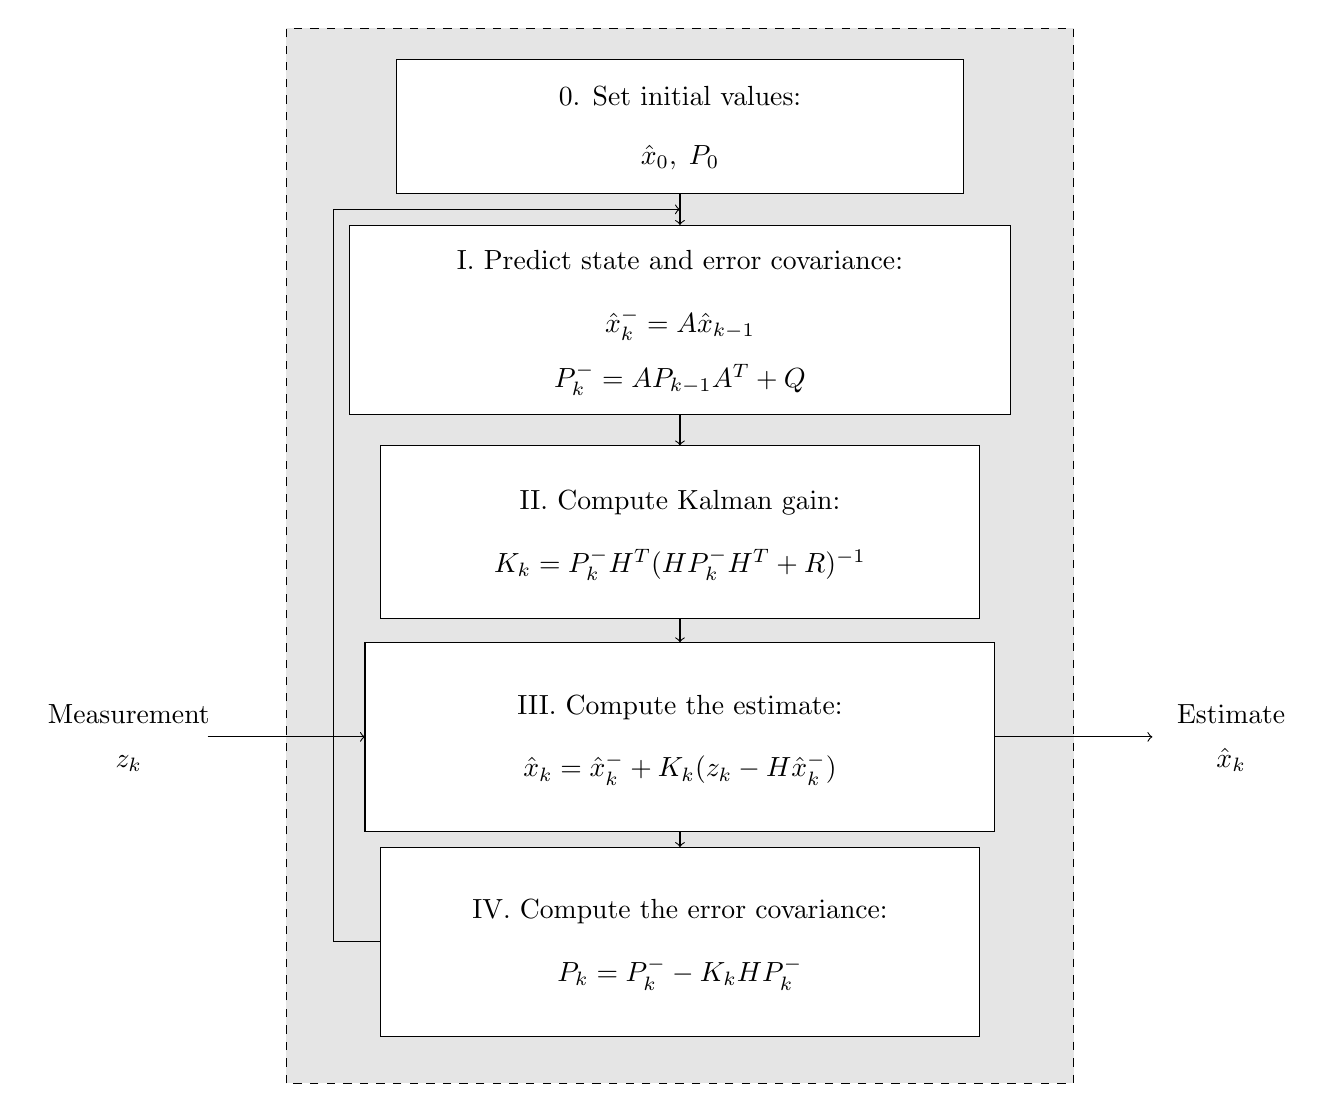
\begin{tikzpicture}

% Fundo externo
\draw[dashed, fill=gray!20]
(-5,-12) rectangle (5,1.4);

% BLOCO 0
\draw[fill=white]
(-3.6,-0.7)
rectangle
(3.6,1.0);

\node at (0,0.15)
{
\begin{tabular}{c}
0. Set initial values:\\[0.2cm]
$\hat{x}_0,\;P_0$
\end{tabular}
};

% BLOCO I
\draw[fill=white]
(-4.2,-3.5)
rectangle
(4.2,-1.1);

\node at (0,-2.3)
{
\begin{tabular}{c}
I. Predict state and error covariance:\\[0.25cm]
$\hat{x}_k^{-}=A\hat{x}_{k-1}$\\[0.15cm]
$P_k^{-}=AP_{k-1}A^T+Q$
\end{tabular}
};

% BLOCO II
\draw[fill=white]
(-3.8,-6.1)
rectangle
(3.8,-3.9);

\node at (0,-5)
{
\begin{tabular}{c}
II. Compute Kalman gain:\\[0.25cm]
$K_k=P_k^{-}H^T(HP_k^{-}H^T+R)^{-1}$
\end{tabular}
};

% BLOCO III
\draw[fill=white]
(-4.0,-8.8)
rectangle
(4.0,-6.4);

\node at (0,-7.6)
{
\begin{tabular}{c}
III. Compute the estimate:\\[0.25cm]
$\hat{x}_k=
\hat{x}_k^{-}
+
K_k(z_k-H\hat{x}_k^{-})$
\end{tabular}
};

% BLOCO IV
\draw[fill=white]
(-3.8,-11.4)
rectangle
(3.8,-9.0);

\node at (0,-10.2)
{
\begin{tabular}{c}
IV. Compute the error covariance:\\[0.25cm]
$P_k=P_k^{-}-K_kHP_k^{-}$
\end{tabular}
};

% SETAS VERTICAIS
\draw[->] (0,-0.7)--(0,-1.1);
\draw[->] (0,-3.5)--(0,-3.9);
\draw[->] (0,-6.1)--(0,-6.4);
\draw[->] (0,-8.8)--(0,-9.0);

% ENTRADA
\draw[->]
(-6,-7.6)
--
(-4,-7.6);

\node at (-7,-7.6)
{
\begin{tabular}{c}
Measurement\\
$z_k$
\end{tabular}
};

% SAÍDA
\draw[->]
(4,-7.6)
--
(6,-7.6);

\node at (7,-7.6)
{
\begin{tabular}{c}
Estimate\\
$\hat{x}_k$
\end{tabular}
};

% REALIMENTAÇÃO
\draw[->]
(-3.8,-10.2)
--
(-4.4,-10.2)
--
(-4.4,-0.9)
--
(0,-0.9);

\end{tikzpicture}

\vspace{0.2cm}

\begin{flushleft}
\footnotesize Source: Adapted from Kim (2011).
\end{flushleft}

\end{figure}

The calculation of the Kalman Gain ($K_k$), the correction of the a posteriori state estimate ($\hat{x}_{k|k}$), and the update of the final covariance matrix ($P_{k|k}$) during this correction phase are defined by:

\begin{equation}
K_k =
P_{k|k-1}
H_k^T
\left(
H_k
P_{k|k-1}
H_k^T
+
R_k
\right)^{-1}
\label{eq:kalman_gain}
\end{equation}

\begin{equation}
\hat{x}_{k|k}
=
\hat{x}_{k|k-1}
+
K_k
\left(
z_k-h(\hat{x}_{k|k-1})
\right)
\label{eq:state_update}
\end{equation}

\begin{equation}
P_{k|k}
=
(I-K_kH_k)
P_{k|k-1}
\label{eq:covariance_update}
\end{equation}

where $K_k$ is the Kalman Gain responsible for weighting the contribution of the predicted estimate and the current measurement; $\hat{x}_{k|k}$ represents the corrected a posteriori state estimate; $P_{k|k}$ denotes the updated error covariance matrix; and $H_k$ is the Jacobian matrix of the nonlinear observation function $h(\cdot)$ \cite{kalman_beginners}.

By acting as this robust predictive estimator in the image plane, the EKF mathematical processing not only attenuates noisy oscillations caused by rotor disturbances and model uncertainty but also compensates for the computational delay introduced by inference, ensuring that the control reference is maintained even during visual frames in which the neural network temporarily fails to detect the target \cite{barisic2019,vidal2007}.

\subsubsecao{Visual Servoing}

In autonomous robotics, Visual Servoing stands out as the fundamental technique for guiding robot motion using visual feedback extracted from one or more cameras, operating in a closed loop \cite{thuilot2002}. In Unmanned Aerial Vehicle (UAV) systems, in which navigation in GPS-denied environments or precise physical interaction (such as robotic gripper locking) requires millimetric reliability, Visual Servoing acts as the direct link between exteroceptive perception and kinematic actuation \cite{shang2016, lopezfranco2017}.

The mathematical premise of Visual Servoing is based on the continuous minimization of an error vector $e(t)$, defined by the difference between the current visual features of the target $s(t)$ and a desired reference state $s^{*}$ \cite{lopezfranco2017, pramono2025}. In order for the reduction of this error to be converted into physical motion, camera kinematics and the variation of visual features are correlated through an Interaction Matrix, also known as the Image Jacobian ($L_s$) \cite{luo2020}. The robot velocity control law is therefore classically formulated through the pseudo-inverse of this matrix ($L_s^{+}$), guaranteeing an exponential decay of the visual error as the aircraft approaches the object \cite{lopezfranco2017, luo2020}.

Historically, the literature consolidates the classification of Visual Servoing schemes into two primary architectures, distinguished by the spatial domain in which the error vector $e(t)$ is computed: Image-Based Visual Servoing (IBVS) and Position-Based Visual Servoing (PBVS) \cite{hutchinson1996, chaumette2016, thuilot2002, hafez2013}.

In the IBVS approach (2D model), the control law operates strictly in the image plane using pixel coordinates \cite{pramono2025}. Although IBVS eliminates the need for a prior three-dimensional model of the target and provides high robustness to intrinsic calibration errors, it presents critical disadvantages in aerial robotics applications. Since the control is projected in pixel coordinates, the trajectory generated in three-dimensional (3D) space is unpredictable \cite{hafez2013, pramono2025, chaumette2016}. Furthermore, due to the phenomenon of mechanical under-actuation, the UAV requires large attitude variations (in roll or pitch) to perform translation \cite{thuilot2002}. Under pure IBVS control, these abrupt attitude changes generate strong dynamic couplings that may drive the controller into local singularities or even cause severe instabilities when target features move outside the camera Field of View (FoV) \cite{hafez2013}.

To mitigate FoV loss caused by aircraft attitude changes, a hardware solution widely adopted in the literature consists of mounting the camera on a stabilized support with independent axes (gimbal) \cite{keipour2022}. Since the gimbal exhibits mechanical response dynamics significantly faster than those of the quadcopter, it actively adjusts lens inclination continuously, isolating the camera from the robot attitude and assisting in retaining the target at the center of the image \cite{keipour2022}. However, the exclusive use of a gimbal does not solve all limitations of aerial Visual Servoing. The addition of this dynamic mechanism makes the mathematical system even more complex, requiring the real-time computation of time-varying transformation matrices to correlate the moving camera reference frame with the chassis control reference frame \cite{keipour2022}. Furthermore, even with the image mechanically stabilized by the gimbal, if the control loop operates purely in the two-dimensional domain (IBVS), the spatial trajectory of UAV approach remains unpredictable, which may generate dangerous overshoots during the critical phase of physical alignment \cite{hafez2013, pramono2025}.

To overcome the remaining algorithmic limitations of IBVS and guarantee greater stability during final robotic gripper alignment, Position-Based Visual Servoing (PBVS --- 3D model) may be adopted. In PBVS, the control objective does not consist solely of generating motion from the direct analysis of pixels but rather reconstructing the geometric pose (distance and orientation) of the target relative to the camera before computing the control effort \cite{thuilot2002, hafez2013}. Figure~\ref{fig:ibvs_pbvs_comparison} illustrates the classical contrast between these two approaches. While IBVS tends to maintain more regular trajectories in the image plane at the cost of potentially inefficient spatial motion, PBVS operates directly in Cartesian metric space, favoring more direct approach trajectories in physical space \cite{pramono2025, fagundes2025, chaumette2016}. As a trade-off, the absence of explicit control over pixel coordinates may cause object features to describe broader trajectories in the image, increasing the risk that the target exceeds the limits of the camera Field of View (FoV) before capture is completed \cite{pramono2025, hafez2013}.

\begin{figure}[H]
    \centering

    \captionsetup{justification=centering}

    \caption{Qualitative comparison between the classical Image-Based Visual Servoing (IBVS) and Position-Based Visual Servoing (PBVS) schemes}
    \label{fig:ibvs_pbvs_comparison}

    \vspace{0.2cm}

    \includegraphics[width=0.75\linewidth]{figuras/ibvs_pbvs_comparison.png}

    \vspace{0.2cm}

    \begin{flushleft}
        \footnotesize Source: Adapted from Hafez et al. (2013).
    \end{flushleft}

\end{figure}

Three-dimensional reconstruction in PBVS schemes is initially based on the application of the analytical Pinhole camera model. This model, geometrically illustrated in Fig.~\ref{fig:pinhole_camera_model}, acts as the bridge between domains by mapping the stabilized two-dimensional coordinates of the target into a three-dimensional vector in the camera focal reference frame through the incorporation of the intrinsic parameters of the lens, such as focal length and optical center \cite{lopezfranco2017, fagundes2025, pramono2025}.

\begin{figure}[H]
    \centering

    \captionsetup{justification=centering}

    \caption{Geometric representation of perspective projection based on the Pinhole camera model, illustrating the relationship between focal length and the conversion of a point in space onto the two-dimensional image plane}
    \label{fig:pinhole_camera_model}

    \vspace{0.2cm}

    \includegraphics[width=1\linewidth]{figuras/pinhole_camera_model.png}

    \vspace{0.2cm}

    \begin{flushleft}
        \footnotesize Source: Björkman (2023), cited in Pramono (2025).
    \end{flushleft}

\end{figure}

Therefore, when adopting the mechanical architecture of a gimbal, the camera reference frame becomes decoupled from the rigid structure of the UAV. However, although the stabilizing support isolates the lens from aircraft attitude changes (preserving the target within the Field of View (FoV)), it introduces a new mathematical complexity: the relative orientation of the camera becomes dynamically time-varying with respect to the robot center of mass \cite{keipour2022}. To cancel this undesired effect and prevent the autonomous rotation of the gimbal from being interpreted by the control loop as target motion, the vector extracted from the Pinhole model must be remapped. This is achieved by multiplying it by cascaded geometric transformation matrices of translation and rotation \cite{fagundes2025, keipour2022}. Using the angular measurements from the gimbal itself and the Inertial Measurement Unit (IMU), these matrices perform instantaneous compensatory rotations, projecting the target coordinates from the moving camera reference frame to the UAV body reference frame and subsequently to an inertial reference frame aligned with the world \cite{fagundes2025, sciortino2018}. This approach concludes the perception pipeline by extracting the position error strictly in translational coordinates expressed in meters.

Since this is a computationally demanding algorithmic pipeline, integrating semantic extraction with neural networks, predictive filtering, Jacobian inversion, and time-varying three-dimensional matrix transformations, the architecture imposes a computational cost that low-level flight controllers alone are generally unable to support \cite{lopezfranco2017}. As an engineering solution, the onboard system may be hierarchically segmented. Thus, the complete computation of the PBVS control loop is executed on an auxiliary onboard computer (companion computer), typically implemented as a node within the ROS (Robot Operating System) ecosystem \cite{shang2016, sciortino2018}. Once the error vector in meters has been computed and converted into velocity signals, the companion computer delegates mechanical execution to the low-level flight controller (such as Pixhawk hardware operating ArduPilot) through the MAVLink/MAVROS serial communication protocol \cite{shang2016, sciortino2018}. This arrangement establishes Visual Servoing as the high-level control system of the UAV, in which vision (assisted by the gimbal) determines the coordinates in three-dimensional space in real time, while the flight controller regulates motor rotation.

\subsubsecao{Aerial Capture and Manipulation Systems}

Historically, the applications of Unmanned Aerial Vehicles (UAVs) were concentrated on the execution of passive observation missions, in which the aircraft acted purely as a remote sensor. The need to interact with and modify the environment motivated the development of Unmanned Aerial Manipulators (UAMs), systems composed of a flying platform coupled with a physical interaction mechanism designed to capture, transport, or manipulate objects \cite{bonyan2018, meng2020}.

According to the state of the art in the aerial manipulation literature, the methods and mechanical systems used to perform capture and physical interaction are divided into four main categories \cite{bonyan2018}:

\begin{itemize}

\item \textbf{Grippers (Figure~\ref{fig:attached_grippers}):} Grippers represent the most common mechanical solution and are ideal for tasks involving purely object capture, payload transportation, and perching operations \cite{meng2020}. Since they are typically compact and lightweight, grippers are installed close to the Center of Mass (CoM) of the UAV, fundamentally operating with two actuation states (open and close). Because they do not require multiple articulation motors, grippers (whether rigid or made of compliant/soft materials) demand lower payload capacity from the aircraft and significantly reduce inertial variations during flight \cite{meng2020, ladig2021}.

\begin{figure}[H]
    \centering
    \captionsetup{justification=centering}

    \caption{Aerial manipulation using attached grippers}
    \label{fig:attached_grippers}

    \vspace{0.2cm}

    \includegraphics[width=0.5\linewidth, angle=180]{figuras/attached_grippers.png}

    \vspace{0.2cm}

    \begin{flushleft}
        \footnotesize Source: Ubellacker et al. (2024).
    \end{flushleft}
\end{figure}

\item \textbf{Articulated Robotic Arms (Figure~\ref{fig:articulated_robotic_arm}):} For missions that require high dexterity rather than only rigid capture, the UAV is equipped with robotic arms ranging from one Degree of Freedom (1-DoF) systems to hyper-redundant manipulators \cite{bonyan2018}. The addition of these articulations expands the operational workspace, allowing the end-effector to reach complex targets, rotate valves, or perform assembly tasks. However, this additional capability introduces the disadvantage of increased weight and continuous displacement of the robot center of gravity with each arm movement \cite{meng2020}.

\begin{figure}[H]
    \centering
    \captionsetup{justification=centering}

    \caption{UAV equipped with an articulated robotic arm}
    \label{fig:articulated_robotic_arm}

    \vspace{0.2cm}

    \includegraphics[width=0.5\linewidth]{figuras/articulated_robotic_arm.png}

    \vspace{0.2cm}

    \begin{flushleft}
        \footnotesize Source: Bonyan Khamseh et al. (2018).
    \end{flushleft}
\end{figure}

\item \textbf{Suspension Cables and Winches (Figure~\ref{fig:cable_suspended_manipulation}):} This method is frequently adopted when capture requires the UAV to operate at a safe distance from the object \cite{ladig2021}. Its use is particularly suitable when the target has low mass or is located in narrow and unstable locations. By maintaining the capture mechanism suspended below the fuselage, the system reduces the effects of downwash, the descending airflow generated by the propellers, preventing the object from being displaced before capture \cite{ladig2021}. However, this approach is more suitable for applications involving tensile forces and presents limitations for operations requiring compressive efforts.

\begin{figure}[H]
    \centering
    \captionsetup{justification=centering}

    \caption{Cable-suspended aerial manipulation system}
    \label{fig:cable_suspended_manipulation}

    \vspace{0.2cm}

    \includegraphics[width=0.5\linewidth, angle=180]{figuras/cable_suspended_manipulation.png}

    \vspace{0.2cm}

    \begin{flushleft}
        \footnotesize Source: Ladig et al. (2021).
    \end{flushleft}
\end{figure}

\item \textbf{UAV Body or Rigid Tools (Figure~\ref{fig:rigid_tool_manipulation}):} In limited manipulation scenarios that do not require grasping the target, the UAV chassis itself or a fixed rigid rod is used to apply direct force, such as pushing objects or performing contact inspection on walls \cite{bonyan2018}.

\begin{figure}[H]
    \centering
    \captionsetup{justification=centering}

    \caption{Rigid-tool aerial manipulation system mounted on the UAV frame}
    \label{fig:rigid_tool_manipulation}

    \vspace{0.2cm}

    \includegraphics[width=0.5\linewidth]{figuras/rigid_tool_manipulation.png}

    \vspace{0.2cm}

    \begin{flushleft}
        \footnotesize Source: Meng et al. (2020).
    \end{flushleft}
\end{figure}

\end{itemize}

In addition to the choice of mechanism, the aerial capture method depends directly on the operational workspace configured in the multirotor chassis. As illustrated in Figure~\ref{fig:interaction_zones}, this geometric configuration divides the robot operational area into three main interaction zones with the environment \cite{ladig2021}:

\begin{itemize}

\item \textbf{Underside Capture:} This is the standard architecture in most aerial robotic projects. The capture mechanism is positioned below the fuselage, configuring the system to retrieve loads located on the ground or on flat platforms below the UAV flight level \cite{ladig2021}.

\item \textbf{Upper-Side Capture:} For high-altitude missions, such as capture on ceilings, tubular structures, and the underside of bridges, the rotors represent a mechanical obstacle for lower-mounted manipulators \cite{ladig2021}. In these cases, grippers and actuators are mounted on top of the UAV. This approach is widely explored for perching operations, allowing the robot to capture a fixed structure above itself, turn off its motors, and save energy while performing inspection tasks \cite{ladig2021, meng2020}.

\item \textbf{Lateral-Side Capture:} Designed to access surfaces and targets vertically aligned with the UAV, such as building facades \cite{ladig2021}. This approach requires extended mechanisms that prevent the rotors from colliding with the wall during approach.

\end{itemize}

Finally, regarding the nature of interaction, these methodologies are unified by the free-flight operational scenario \cite{meng2020}. In this context, physical contact with the environment should last for the shortest possible time, such that, in the task of aerial target capture, the closure of the mechanism (gripper or arm) is characterized as a rapid and discrete mechanical event. Consequently, it is the combination between the selected actuation method (gripper, arm, or winch) and the operational workspace that determines the technical capability of the UAV to isolate and safely grasp a target under non-cooperative conditions \cite{meng2020}.

\begin{figure}[H]
    \centering
    \captionsetup{justification=centering}

    \caption{Classification of operational spaces in aerial manipulation systems}
    \label{fig:interaction_zones}

    \vspace{0.2cm}

    \includegraphics[width=0.4\linewidth]{figuras/interaction_zones.png}

    \vspace{0.2cm}

    \begin{flushleft}
        \footnotesize Source: Ladig et al. (2021).
    \end{flushleft}
\end{figure}

\subsecao{Related Works}

\subsubsecao{Autonomous Object Capture by UAVs}

In the article titled \textit{Toward Image Based Visual Servoing for Aerial Grasping and Perching}, Thomas et al.~\cite{thomas2014} developed a system enabling small drones to autonomously approach and land on cylindrical structures, a maneuver known as perching. Inspired by the way birds land on branches, the study avoided overloading the UAV with heavy motors. Instead, the authors installed a simple gripper at the base of the aircraft. This gripper used the UAV’s own velocity and the impact force with the target to close rapidly, securing the object without the need for additional electrical actuators.

To ensure that the drone hit the target accurately, the project employed Image-Based Visual Servoing (IBVS) assisted by a laboratory camera system (MOCAP) in an indoor environment. The main technological challenge of this approach was ensuring that the control system reacted fast enough to stabilize the drone at the exact moment the gripper contacted the cylinder. At this contact instant, the UAV transitioned from free flight to a state subjected to a strong physical impact disturbance.

The experimental results reported by Thomas et al.~\cite{thomas2014} successfully validated this bio-inspired approach. Operating a lightweight quadrotor of 388 grams equipped with a 478-gram gripper, the visual servoing architecture demonstrated the ability to grasp and transport 77-gram symmetric loads in free flight with high stability. In addition to proving the accuracy of the vision system, the strategy enabled complete shutdown of the motors after gripper engagement, resulting in significant energy savings while the robot operated as a suspended observation platform.

In the article titled \textit{Autonomous Marker-less Rapid Aerial Grasping}, Bauer et al.~\cite{bauer2023} developed a system focused on solving the problem of fast object capture in the air without the use of artificial markers. The main objective of the project was to create a quadrotor capable of identifying, approaching, and grasping targets in a fully autonomous manner under non-cooperative conditions. To prevent damage to the aircraft during high-speed physical impact, the authors equipped the UAV base with a soft and flexible robotic gripper designed to passively conform to the object shape.

To enable marker-less detection, the system used an onboard depth camera. The video stream was transmitted in real time to an external high-performance processing station (equipped with an RTX-3070 GPU). On this computer, a deep learning neural network based on image segmentation (Mask R-CNN) identified the object contour. The algorithm then fused these detections with depth camera data to generate a 3D map (point cloud) of the target, accurately estimating its geometry and determining optimal grasping points for gripper closure.

The experimental results demonstrated the feasibility of combining intelligent vision with compliant mechanical design. During free-flight experiments, the perception system was able to guide the UAV toward the target, while the natural flexibility of the soft gripper absorbed mechanical impact and compensated for small inevitable pose estimation errors. This approach achieved a capture success rate of 89\% in aerial grasping trials. This metric confirms that fast and reliable aerial grasping is possible even when the environment or the target does not cooperate with the robot vision system.

In the article titled \textit{High-speed aerial grasping using a soft drone with onboard perception}, Ubellacker et al.~\cite{ubellacker2024} aimed to develop a UAV capable of performing autonomous high-speed aerial grasping using only onboard perception. The project goal was to eliminate dependency on external infrastructure, such as motion capture (MOCAP) camera laboratories. To ensure safety during high-speed impact, the researchers introduced a soft robotic gripper designed to deform, absorb shock, and passively conform to the target at the exact moment of capture.

To enable marker-less perception, the visual system combined neural networks and depth sensors. First, an artificial intelligence model analyzed camera images to detect key points (object silhouette). Then, the onboard computer fused these detections with depth data to estimate the precise three-dimensional (3D) position and orientation of the target, allowing the UAV to autonomously plan its approach trajectory.

The experimental results validated the integration of onboard 3D vision and soft grippers. Flying at an approach speed of 0.5 m/s, the UAV achieved a perfect success rate of 10 out of 10 trials for bottle grasping, and 9 out of 10 trials for a medical kit. The system also demonstrated versatility by successfully performing grasps in outdoor environments. Furthermore, the study identified operational limits of the platform: when the capture speed was increased beyond 2.0 m/s, the success rate for the bottle dropped to only 3 out of 10 trials (30\%). This result highlights that, although the compliant gripper compensates for small pose errors, the system performance degrades under high-speed operation due to increased visual estimation error.

In the article titled \textit{Natural Feature-based Visual Servoing for Grasping Target with an Aerial Manipulator}, Luo et al.~\cite{luo2020} proposed an aerial manipulation architecture guided exclusively by natural visual features of the target. The main objective was to eliminate the need for cooperative artificial markers such as QR codes, ArUco tags, or reflective stickers. Instead, the UAV had to perform tracking by identifying only the natural textures and edges of the target itself. The system used a lightweight custom-built 6-DoF robotic arm attached to the UAV base to perform precision grasping.

To implement this idea, the method decomposed the task into stages, combining UAV flight control with robotic arm motion. The authors mounted a standard camera on the end-effector of the robotic arm and used an onboard minicomputer (Intel NUC) for image processing. The algorithm was designed to extract and track salient feature points of the target using the ORB feature detection method. Based on these points, the system computed the pixel displacement of the object and directly converted this visual information into velocity commands to drive the robotic arm motors autonomously and in real time.

The experimental results confirmed the maturity and efficiency of this contour-based visual approach. During practical tests, the aircraft was able to identify the target and initiate a fully autonomous approach from a distance of 3 meters. When the UAV reached 0.4 meters (40 centimeters) from the object, it stabilized in hover and fully transferred visual control to the robotic arm (which weighed only 0.9 kg). The camera guided the fine approach until a distance of 20 centimeters from the target was reached, at which point the system triggered the mechanical closure and successfully completed the grasp.

\subsubsecao{Object Detection and Tracking in UAVs}

In the article titled \textit{Vision-based system for a real-time detection and following of UAV}, Barisic et al.~\cite{barisic2019} developed a system enabling a UAV to detect, track, and follow another drone in real time. The challenge of this research was to maintain a fast-moving aerial object, subject to abrupt changes in altitude and direction, centered in the follower UAV camera image during fully autonomous flight.

To implement the system, the authors combined artificial intelligence with a Kalman Filter. In the vision stage, they trained a neural network (YOLOv3-Tiny) using a custom dataset composed of 10,000 drone images. The detection ran directly on the onboard computer of the aircraft. However, the size of the bounding box generated by the neural network around the target exhibited jitter due to propeller-induced disturbances. To stabilize perception, the system employed a Kalman Filter to track eight continuous variables: the center coordinates, width, and height of the bounding box, as well as the velocities of all these quantities. In this way, even if the camera temporarily lost sight of the target, the filter could predict the exact location and size of the drone in space.

The experimental results demonstrated the success of integrating intelligent vision with predictive filtering. The camera processing operated at 20 frames per second (FPS), achieving a mean Average Precision (mAP) of 97.88\% in detections. Although the original paper primarily validates the Kalman Filter through graphical results, the experiments confirm that its application was essential. By smoothing unstable bounding box measurements, the filter ensured that the follower UAV kept the target centered even when the tracked drone performed complex figure-eight maneuvers, enabling continuous and collision-free tracking.

In the article titled \textit{Vision-based system for a real-time detection and following of UAV}, Barisic et al.~\cite{barisic2019} developed a vision-based system enabling a UAV to detect, track, and follow another multirotor in real time. The main challenge of this study was to keep a fast-moving aerial object, subject to abrupt changes in altitude and direction, centered in the camera field of view during fully autonomous flight.

To solve this problem, the authors proposed the integration of convolutional neural networks with the Kalman Filter. In the visual perception stage, they employed the YOLOv3-Tiny model, trained using a custom dataset composed of 10,000 UAV images, running directly on the aircraft onboard computer. However, the authors reported that the dimensions of the bounding box generated by the neural network exhibited oscillations and significant variations due to the rapid rotation of the target propellers. To mitigate this visual volatility, the system applied a Discrete Kalman Filter responsible for tracking eight continuous states: the center coordinates, the width and height of the bounding box, as well as their respective velocities. In this way, even in cases of occlusion and temporary loss of detection, the filter was able to predict the drone’s spatial location and size.

The experimental results validated the effectiveness of integrating deep learning-based perception with predictive filtering. The onboard processing operated at a rate of 20 frames per second (FPS), achieving a mean Average Precision (mAP) of 97.88\% in detections. The effectiveness of the Kalman Filter application is graphically shown in Fig.~\ref{fig:kalman_barisic_results}. By smoothing fluctuations and jittering bounding box measurements into a continuous predictive estimate, the filter ensured that the follower UAV computed control references and kept the target continuously centered, even when the tracked aircraft executed complex three-dimensional figure-eight maneuvers, enabling robust and collision-free tracking \cite{barisic2019}.

\begin{figure}[H]
    \centering
    \captionsetup{justification=centering}

    \caption{Comparison between Kalman Filter estimation and object detection output for the width and height of the bounding box}
    \label{fig:kalman_barisic_results}

    \vspace{0.2cm}

    \includegraphics[width=0.8\linewidth]{figuras/kalman_barisic_results.png}

    \vspace{0.2cm}

    \begin{flushleft}
        \footnotesize Source: Barisic et al. (2019).
    \end{flushleft}
\end{figure}

In the article titled \textit{Object Visual Tracking using Window-Matching Techniques and Kalman Filtering}, Vidal and Casanova~\cite{vidal2007} proposed a robust predictive method for tracking moving objects in video sequences. The focus of the study was to address the problem of ``camera drift'', a common failure in which the vision system becomes confused, gradually loses the true target, and starts tracking background regions or image shadows.

To solve this problem, the authors developed an algorithm combining visual search through Window-Matching techniques with the Kalman Filter. The vision system extracted image patches (regions of interest) using sliding windows (50$\times$50 or 15$\times$15 pixels) and mathematically computed which region in the next video frame most closely matched the target. To prevent errors when image quality degraded, the Kalman Filter was integrated into the pipeline. Thus, when the camera produced a false positive or the object became temporarily occluded, the Kalman prediction took priority, constraining the search area and estimating the target position based on its previously observed motion and velocity.

The experimental results confirmed the effectiveness of this combined approach for correcting tracking failures. Although the original study mainly presents graphical results, tests using 320$\times$240 resolution videos demonstrated the superiority of the filtering approach. When tracking a vehicle at an urban intersection, partially occluded pedestrians, and a floating bottle in the sea (a highly cluttered and unstructured background), the vision-only algorithm quickly failed. However, with the addition of the Kalman Filter, the system compensated for uncertainties, reduced pixel drift, and maintained a smooth and stable trajectory on the target, demonstrating the effectiveness of predictive filtering in dynamic environments.

In the article titled \textit{DS-YOLOv8-Based Object Detection Method for Remote Sensing Images}, Shen et al.~\cite{shen2023} aimed to detect very small objects for monitoring using drone cameras and aerial imagery. The challenge of this study lies in the fact that, from high altitudes, objects lose their fine details and appear as small pixel clusters in the image. This causes traditional vision algorithms, trained on close-range scenarios, to frequently fail in classification tasks.

To address this issue, the researchers proposed the DS-YOLOv8 algorithm, an artificial intelligence model that modifies and improves the eighth version of the YOLO family. To compensate for the lack of resolution, they redesigned the internal network architecture by splitting image processing into smaller and more efficient channels. The goal of these modifications was to extract visual features in greater detail, preserving the shape information of small objects during processing while maintaining a lightweight and fast model suitable for real-time execution.

The experimental results demonstrated improved reliability in aerial vision tasks. The DS-YOLOv8 model achieved a mean Average Precision (mAP) of 91.0\% and an F1-score of 90.4\% for detecting small and distant targets. Despite these results, the study also identified limitations, showing that performance degrades in scenarios where objects are extremely densely clustered. Nevertheless, the reported metrics indicate that the modified architecture is highly effective and well-suited for aerial inspection platforms.

Finally, exploring computer vision in space, the article titled \textit{A Space Non-Cooperative Target Recognition Method for Multi-Satellite Cooperative Observation Systems}, developed by Zhang et al.~\cite{remotesensing2024}, aimed to identify and locate multiple non-cooperative targets, such as defunct satellites and space debris. The challenge of this research was to correct a common error in which the system detects parts of the same object as independent targets. Since the camera observes solar panels separated from the main body of the satellite, the algorithm would draw multiple redundant bounding boxes over the same object, fragmenting the image and misleading the control system of the pursuing platform.

To solve this problem, the authors developed a high-efficiency detection model divided into two stages, named LCNN-DMT. In the first stage, they proposed the MBRT-D algorithm, which analyzes the spatial distribution of bounding boxes on the image. If the boxes drawn around a solar panel and the satellite body are too close (below a defined distance threshold), the system automatically merges them into a single bounding box, ensuring that the object is fully represented. In the second stage, this unified and cleaned representation is processed by a lightweight neural network (based on SqueezeNet), enhanced with attention mechanisms to focus on the most relevant features and quickly classify whether the object is a satellite or space debris.

The experimental results demonstrated the success of this approach. The bounding-box merging strategy completely eliminated fragmentation issues, providing reliable target localization. In numerical terms, the LCNN-DMT network achieved a mean Average Precision (mAP) of 97.50\%. When compared with established detection algorithms, it significantly outperformed Faster R-CNN (89.17\%) and its previous baseline model T-SCNN (86.64\%). In addition to accuracy improvements, the model demonstrated high computational efficiency, processing images in only 6.1 milliseconds. Requiring only 0.928 million parameters and consuming just 0.464 GFLOPs, the study confirmed that this architecture is well suited for deployment on companion computers with severe power and computational constraints.

\subsubsecao{Visual Servoing Applied to UAVs}

In the dissertation titled \textit{Hybrid PBVS-IBVS Model Predictive Visual Servoing For Autonomous Docking of a Free-Flying Robot}, Tafarrel Firhannoza Pramono~\cite{pramono2025} aimed to develop a hybrid visual servoing method for autonomous docking of aerial robots. The objective was to combine the strengths of two visual control approaches: preventing the camera from losing sight of the target (a critical issue when the robot relies solely on 2D image tracking) while also correcting the precision and geometric calibration errors that arise when estimating the object pose exclusively in 3D space.

The system was developed and tested in simulation environments (such as ROS and Gazebo) and validated on real free-flying robotic platforms. The UAV was equipped with a depth camera capable of generating 3D point clouds. To enable real-time onboard processing, filtering techniques were applied to remove irrelevant points and reduce computational load. The onboard system used a Model Predictive Controller (MPC), which anticipates future states and dynamically blends navigation strategies: the UAV uses 3D vision for long-range approach (where the error is larger) and gradually switches to 2D image-based control when it is close to the target, enabling precise docking.

The practical and simulation results validated the performance of this smooth control transition. During laboratory validation tests (with real hardware), the robot was able to perform autonomous in-motion docking with success rates ranging from 80\% to 100\% of the trials, tracking the target from an initial distance greater than 1.5 meters. The computational performance also proved effective, with visual tracking running at 30 frames per second (30 Hz) and the flight controller updating trajectories at 15 Hz. Regarding docking impact accuracy, the robot’s steady-state error was nearly zero, achieving a spatial precision of only 1 millimeter position deviation and 0.25 degrees attitude deviation. These results demonstrate that combining the best of 2D and 3D techniques not only keeps the target within the camera field of view at all times but also enables extremely precise and smooth docking, even when the UAV starts fully misaligned with the target.

In the article titled \textit{Fractional Order Robust Visual Servoing Control of A Quadrotor UAV with Larger Sampling Period}, Shang et al.~\cite{shang2016} aimed to design a highly robust control system to ensure that a drone could maintain stable hovering. The practical problem addressed by the study was computational delay: since small onboard computers are slow in processing images, they output only a few frames per second (low FPS). This delay creates a “visual lag”, which directly conflicts with the fast physical dynamics of the UAV, causing instability and oscillatory behavior or even loss of control.

To solve this problem, the authors proposed a control strategy beyond classical approaches, adopting a Fractional-Order Proportional-Derivative (FOPD) controller. In simple terms, fractional calculus introduces additional flexibility that allows the system to absorb and compensate for video delay more smoothly. On the hardware side, the system strictly separates tasks: an onboard companion computer handles the computationally heavy perception stage (even at low frame rates) and sends target coordinates to a main flight controller, which focuses exclusively on stabilizing motor outputs and maintaining UAV attitude and altitude.

The experimental tests, conducted at a flight altitude of 10 meters, demonstrated that FOPD control outperforms traditional PID controllers under delay conditions. During experiments, the system was forced to operate with an extremely large image delay period of 0.58 seconds per frame. Even while effectively operating with more than half a second of visual delay between processed frames, the fractional-order controller compensated for the lag and kept the UAV stabilized over the target within a maximum deviation radius of only 58 pixels in the image. In direct comparison, the classical PID controller exhibited oscillations and deviations reaching a radius of 68 pixels. These results confirm that fractional-order control improves flight stability by approximately 20\%, ensuring accurate performance without requiring high-cost, high-performance onboard processors.

In the article titled \textit{Visual Servoing Using Sliding-Mode Control with Dynamic Compensation for UAVs' Tracking of Moving Targets}, researchers Carvajal et al.~\cite{carvajal2024} developed a system enabling a UAV to continuously track and follow a moving ground target. The challenge of this research was not only to follow the object in the image but also to ensure the simultaneous fulfillment of safety tasks, such as maintaining a constant safe distance between the drone and the target, and fixing the flight orientation so that the aircraft flew in the same direction as the pursued vehicle.

To put this idea into practice, the system was structured using the Sliding-Mode Control (SMC) technique and divided into two actuation stages. In the first stage, the software processed the camera images at a rate of 50~frames per second (50~Hz) to identify the target (a ground robot with a red spherical marker) and converted its position on the screen into velocity commands for the drone. However, in the second stage, to prevent the drone from lagging behind or losing sight of the target due to its own flight inertia, the authors added a ``dynamic compensator''. This second controller worked by predicting the ground target's acceleration and velocity, which allowed for the correction and anticipation of the UAV's motor commands to prevent response delays.

Field operational trials proved the effectiveness of this compensating system in eliminating delays and stabilizing the aircraft. In one of the most challenging practical experiments, the ground robot performed figure-eight maneuvers for 120~seconds continuously, while the drone was commanded to follow it, maintaining a distance of exactly 2.5~meters. The results demonstrated that the dynamic compensator rejected external disturbances (such as wind) and kept the UAV's maneuvering velocity errors extremely close to zero. Ultimately, the UAV complied with the parameters required by the safety tasks, keeping the target centered in the camera lens at all times, thereby proving the robustness of the Sliding-Mode technique for tracking fast objects in practice.

In the article titled \textit{Visual Servoing for an Autonomous Hexarotor Using a Neural Network Based PID Controller}, researchers Lopez-Franco et al.~\cite{lopezfranco2017} aimed to develop an intelligent visual system to keep a six-rotor drone (hexarotor) perfectly aligned and hovering over a target. The challenge of the study was to solve the problems associated with traditional controllers. Because standard controllers have fixed flight rules, they fail and lose control of the aircraft when the system faces uncertainties, such as sudden changes in the robot's weight or delays in camera image processing.

To resolve these failures, the authors created a hybrid system that combined purely two-dimensional visual tracking (on the camera image plane) with an Artificial Neural Network connected directly to a classical controller, forming a Neural PID (PID-ANN). In simple terms, the onboard computer analyzed the error between the target's position on the screen and the center of the lens. Instead of calculating the movement using complex geometric equations or rigid correction values previously programmed, the neural network's intelligence used this visual error to ``learn'' the new dynamics of the robot and automatically readjust the motor forces in milliseconds, actively adapting to the environment.

Practical and simulation results attested to the stability gain provided by this continuous adaptation. During testing, the researchers forced severe uncertainties on the robot, such as a sudden 50\% increase in its mass and drastic changes to its mechanical inertia. Under these conditions, the classical control (standard PID) could not adapt to the new weight; it became destabilized and diverged from the target, accumulating an error of up to 1741~pixels of deviation in the image. In contrast, under the same conditions, the Neural PID adapted its rules instantly, held the aircraft at the center of the target, and contained the maximum deviation to just 212~pixels. These figures prove that the neural network can compensate for the physical losses of the UAV, ensuring millimeter-accurate tracking without the need to process the complex 3D reconstruction of the world.

\subsubsecao{Comparative Analysis of Related Works}

In order to substantiate the methodological choices of this work, Table~\ref{tab:correlatos} presents a comprehensive comparative summary of the main research developed in the field of autonomous aerial manipulation and target tracking. This literature survey systematically highlights the specific visual perception strategies, applied control techniques, and mechanical capture mechanisms adopted in each referenced study. By analyzing these diverse approaches, the table contrasts their most significant practical results against the operational limitations inherent to each system, such as environmental dependencies and computational constraints. Through this detailed mapping, special emphasis is placed on critical operational challenges, notably autonomous flight alignment, dynamic inertia compensation, and visual processing latency. Consequently, this evaluation not only clarifies the current state of the art but also provides a solid theoretical foundation to justify the specific control and computer vision architecture proposed in the subsequent sections of this research.

\renewcommand{\arraystretch}{1.3} 
\footnotesize 

% Encolhe o espaço em branco entre as colunas (o padrão é 6pt)
\setlength{\tabcolsep}{4pt} 

% O @{} nas pontas arranca a margem invisível externa da tabela
\begin{longtable}{
    @{} 
    >{\raggedright\arraybackslash}p{0.10\textwidth} 
    >{\raggedright\arraybackslash}p{0.16\textwidth} 
    >{\raggedright\arraybackslash}p{0.14\textwidth} 
    >{\raggedright\arraybackslash}p{0.12\textwidth} 
    >{\raggedright\arraybackslash}p{0.20\textwidth} 
    >{\raggedright\arraybackslash}p{0.18\textwidth}
    @{} 
}
    \caption{Comparative Analysis of Related Works}
    \label{tab:correlatos} \\
    \hline
    \textbf{Author (Year)} & \textbf{Detection and Tracking} & \textbf{Control Technique} & \textbf{Capture Mechanism} & \textbf{Study Limitations} & \textbf{Main Results} \\ \hline
    \endfirsthead

    % --- CABEÇALHO PARA AS PÁGINAS SEGUINTES ---
    \multicolumn{6}{c}{{\tablename\ \thetable{} -- continued from previous page}} \\
    \hline
    \textbf{Author (Year)} & \textbf{Detection and Tracking} & \textbf{Control Technique} & \textbf{Capture Mechanism} & \textbf{Study Limitations} & \textbf{Main Results} \\ \hline
    \endhead

    % --- RODAPÉ PARA O FINAL DA PÁGINA (QUANDO QUEBRA) ---
    \hline \multicolumn{6}{r}{{Continued on next page}} \\
    \endfoot

    \hline
    \multicolumn{6}{@{}l}{Source: Prepared by the author (2026).} \\
    \endlastfoot

    % --- CONTEÚDO DA TABELA ---
    Thomas et al. (2014) & External cameras (MOCAP) / Visual Servoing (IBVS) & Post-impact reactive stabilization & Simple base gripper (impact closure) & Total dependence on laboratory with cameras (indoor). Does not work in outdoor environments. & Successful 77g perching; major battery savings. \\ \hline
    
    Bauer et al. (2023) & Onboard visual perception (Marker-less) & Not detailed (autonomous approach) & Soft/flexible robotic gripper & Undamped impact at high speed requires maneuvering restrictions. & 89\% success rate in free flight; mechanical compensation of visual error. \\ \hline
    
    Ubellacker et al. (2024) & Onboard 3D vision & Not detailed & Soft robotic gripper (shock absorption) & Drastic drop in accuracy (30\% success) at speeds over 2.0~m/s due to visual error. & 100\% success at 0.5~m/s in capturing bottles and medical kits. \\ \hline
    
    Luo et al. (2020) & Natural visual features (edges/textures) & Multi-task Visual Servoing (IBVS/PBVS) & Lightweight 0.9~kg robotic arm (6-DoF) & Addition of excessive weight; requires the target to have very clear textures. & Autonomous capture at 3~m, flight stabilization at 0.4~m, and actuation at 20~cm. \\ \hline
    
    Barisic et al. (2019) & YOLOv3 Tiny + Discrete Kalman Filter & Visual Servoing (Active pursuit / Following) & N/A (Only pursuit of another UAV) & The bounding box jitters aggressively due to camera/propeller movement. & mAP of 97.88\% at 20~FPS; robust tracking even with the target performing figure-eight maneuvers. \\ \hline
    
    Vidal \& Casanova (2007) & Window-Matching + Kalman Filter & N/A (Predictive computer vision only) & N/A (Video tracking) & Without the Kalman Filter, the classical algorithm suffers from ``camera drift'' and loses the target to the image background. & Compensated for visual failures, partial occlusions, and dynamic backgrounds (e.g., bottle in the sea). \\ \hline
    
    Shen et al. (2023) & DS-YOLOv8 (Focus on small/aerial targets) & N/A (Remote detection) & N/A & Performance drops significantly when targets are densely clustered. & mAP of 91.0\% and F1-Score of 90.4\% on very distant targets. \\ \hline
    
    Zhang et al. (2024) & LCNN-DMT (SqueezeNet + Attention Mechanism) & N/A (Spatial Recognition) & N/A & Initial tendency of the network to fragment the target by drawing multiple separate boxes. & mAP of 97.50\%; extremely fast execution in only 6.1~milliseconds (Low-SWaP). \\ \hline
    
    Pramono (2025) & Hybrid Visual Servoing & Model Predictive Control (MPC) & Docking (Autonomous physical coupling) & Mathematical / geometric complexity in handling camera matrices. & Combined the 3D rectilinear trajectory of PBVS without letting the target escape the image edges (IBVS). \\ \hline
    
    Shang et al. (2016) & Low-frequency visual servoing (delayed image) & Cascaded FOPD Controller (Fractional Order) & N/A (Focus on hovering) & Severe processor latency limits maneuvers; classical PID control would not withstand it. & Stabilized flight under absurd image delays (0.58s), maximum deviation of only 58~pixels. \\ \hline
    
    Carvajal et al. (2024) & 50Hz Camera (color/sphere tracking) & Sliding-Mode Control (SMC) + Dynamic Compensator & N/A (Ground vehicle tracking) & Strong inertia; the drone would lose the target without the dynamic velocity compensator. & Anticipated acceleration and commands to avoid tracking delays. \\ \hline
    
    Lopez-Franco et al. (2017) & Visual Servoing (Alignment over the target) & Neural PID (adaptive) & N/A (Hover over target) & Classical controllers diverge absurdly (1741~pixels) upon unmodeled disturbances. & Contained the error to 212~pixels even after a surprise 50\% increase in UAV weight. \\
\end{longtable}

The analysis of related works indicates that autonomous aerial manipulation has shown significant advancements in specific subsystems; however, limitations still exist regarding the integration of these components into complete architectures capable of operating exclusively with real-time onboard perception. Pioneering works, such as that by Thomas et al.~\cite{thomas2014}, have demonstrated the mechanical viability of strategies like perching and underside capture using passive grippers. However, the reliance on external motion capture systems (MOCAP) restricts these solutions to controlled laboratory environments.

Aiming to expand the applicability of these approaches to unstructured and GPS-denied environments, various studies began to explore the use of onboard computer vision based on perception that does not require markers such as ArUco. In this context, the results presented by Bauer et al.~\cite{bauer2023} and Ubellacker et al.~\cite{ubellacker2024} highlight the viability of capturing dynamic targets using exclusively onboard sensors.

Within this scenario, the methods employed for extracting visual information become a central component of the system. Traditional techniques based on natural features present limitations related to computational cost and scalability~\cite{luo2020}. Conversely, recent studies indicate the consistent performance of Convolutional Neural Networks in visual detection tasks. The results obtained by Shen et al.~\cite{shen2023} and Zhang et al.~\cite{remotesensing2024} show that modern architectures can maintain high levels of precision (mAP) with computational costs compatible with onboard applications. Considering the requirements of this project, such evidence supports the choice of the YOLO architecture (v8n/v11n) as the primary detection method, aiming to perform the semantic isolation of the cage at high processing rates without compromising the resources available on the companion computer.

Nevertheless, the literature also indicates that the outputs produced directly by detection models are generally not suitable for immediate use in the control loop. As observed by Barisic et al.~\cite{barisic2019}, visual tracking in UAVs can generate bounding boxes subject to noise and instabilities resulting from structural vibration and partial occlusions caused by the propellers. In this regard, both the results presented by Barisic et al.~\cite{barisic2019} and the studies by Vidal and Casanova~\cite{vidal2007} reinforce the use of state estimation techniques to smooth and predict the observed motion. Thus, in this project, an Extended Kalman Filter (EKF) will be adopted, aiming to reduce oscillations in the pixel coordinates and maintain continuous estimates during temporary losses of tracking.

Finally, regarding dynamic control, studies focused on visual servoing highlight limitations associated with exclusively image-based control (IBVS). Pramono~\cite{pramono2025} and Carvajal et al.~\cite{carvajal2024} argue that spatial reconstruction for the three-dimensional domain (PBVS) tends to produce more predictable trajectories suitable for approach and docking operations. Furthermore, Shang et al.~\cite{shang2016} showed that delays between visual acquisition and inertial measurements can introduce effects that degrade the controller's performance. Therefore, the analyzed works substantiate the architecture proposed in this study, based on the conversion of filtered 2D coordinates into 3D metric coordinates using the Pinhole model, and the subsequent use of this error in a cascaded PD controller, aiming to provide greater stability during the approach and to reduce the effects of delays associated with visual processing.